\chapter{Results}
Three test cases were performed over idealised terrain in two dimensions.  First, we examine the accuracy of the upwind-biased advection scheme with the horizontal advection of a scalar tracer.  Second, the results of horizontal advection are compared with tracer advection in a velocity field that follows the terrain.  Third, spurious flow and energy conservation are examined for a stable atmosphere initially at rest.  Fourth, hydrostatic gravity waves in an isothermal atmosphere are forced by flow over terrain.  Results reveal errors in potential temperature near the ground.  Fifth, the same vertical potential temperature profile is advected using another terrain-following velocity field to isolate the cause of the errors seen in the gravity waves test.

For each test, results on BTF, SLEVE and the cut cell style `SnapCol' grid are compared.  Tests that use terrain following velocity fields omit results for the SLEVE grid.

\section{Horizontal tracer advection}
\label{sec:advection}

Following \textcite{schaer2002}, a tracer is transported above the orography by solving the advection equation for a prescribed horizontal wind.  This challenges the accuracy of the advection scheme in the presence of grid distortions.
The wind profile, terrain profile and initial tracer field are shown in Figure~\ref{fig:advection:initial}.

\subsection{Specification}
The domain is \SI{300}{\kilo\meter} wide and \SI{25}{\kilo\meter} high.  The terrain is wave-shaped, specified by the surface height $\surface$ such that
\begin{subequations}
\label{eqn:advection:schaerCos}
\begin{align}
	\surface(x) &= \cos^2 \left( \frac{\pi x}{\lambda} \right) \surface^\star
%
	\intertext{where}
%
	\surface^\star(x) &= \left\{ \begin{array}{l l}
		h_0 \cos^2 \left( \frac{\pi x}{2a} \right) & \quad \text{if $| x | < a$} \\
		0 & \quad \text{otherwise}
	\end{array} \right.
\end{align}
\end{subequations}
where $a = \SI{25}{\kilo\meter}$ is the mountain half-width, $h_0 = \SI{3}{\kilo\meter}$ is the maximum mountain height, and $\lambda = \SI{8}{\kilo\meter}$ is the wavelength.  On the SLEVE grid, the large-scale component $\surface_1$, as described in section~\ref{sec:theory:tf}, is given by
\begin{align}
	\surface_1(x) &= \frac{1}{2}\surface^\star(x)
\end{align}
and $s_1 = \SI{15}{\kilo\meter}$ is the large scale height, and $s_2 = \SI{2.5}{\kilo\meter}$ is the small scale height.  The optimisation of SLEVE by \textcite{leuenberger2010} is not used, so the exponent $n = 1$.

For comparison, the same tests were performed with no orography, such that $\surface = \SI{0}{\kilo\meter}$ everywhere.

The wind is entirely horizontal and is prescribed as
\begin{align}
	u(z) = u_0 \left\{ \begin{array}{l l}
		1 & \quad \text{if $z \geq z_2$} \\
		\sin^2 \left( \frac{\pi}{2} \frac{z - z_1}{z_2 - z_1} \right) & \quad \text{if $z_1 < z < z_2$} \\
		0 & \quad \text{otherwise}
	\end{array} \right.	
\end{align}
where $u_0 = \SI{10}{\meter\per\second}$, $z_1 = \SI{4}{\kilo\meter}$ and $z_2 = \SI{5}{\kilo\meter}$.
This results in a constant wind aloft, and zero flow at \SI{4}{\kilo\meter} and below.
A tracer $\varphi$ is positioned upstream above the height of the terrain.  It has the shape
\begin{align}
	\varphi(x, z) &= \varphi_0 \left\{ \begin{array}{l l}
		\cos^2 \left( \frac{\pi r}{2} \right) & \quad \text{if $r \leq 1$} \\
		0 & \quad \text{otherwise}
	\end{array} \right.
%
\intertext{having radius $r$ given by}
%
	r &= \sqrt{
		\left( \frac{x - x_0}{A_x} \right)^2 + 
		\left( \frac{z - z_0}{A_z} \right)^2
	}
\end{align}
where $A_x = \SI{25}{\kilo\meter}$, $A_z = \SI{3}{\kilo\meter}$ are the horizontal and vertical half-widths respectively, and $\varphi_0 = 1$ is the maximum magnitude of the anomaly.  At $t = \SI{0}{\second}$, the anomaly is centred at $(x_0, z_0) = (\SI{-50}{\kilo\meter}, \SI{9}{\kilo\meter})$ so that the anomaly is upwind of the mountain and well above the maximum terrain height of \SI{3}{\kilo\meter}.  Analytic solutions can be found by adjusting the anomaly centre such that $x_0 = ut$.

\begin{figure}
	\centerfloat
	\input{advection-initial-plot}
	\caption{Vertical cross section of the two-dimensional advection test showing the horizontal wind profile, surface terrain profile and tracer field at $t = \SI{0}{\second}$ on a $\SI{300}{\kilo\meter} \times \SI{25}{\kilo\meter}$ domain.  Adapted from \textcite{schaer2002}.}
	\label{fig:advection:initial}
\end{figure}

\subsection{Discretisation}
The OpenFOAM solver \shellcmd{scalarTransportFoam} was used to implicitly solve the advection equation in flux form
\begin{align}
	\frac{\partial \varphi}{\partial t} + \del \cdot \left( \vect{u} \varphi \right) = 0 \label{eq:advection:continuous}
\end{align}

The time derivative ($\partial \varphi / \partial t$) is solved implicitly using a backward-in-time, second order accurate scheme defined as \autocite{openfoam-progguide}
\begin{align}
	\frac{\partial}{\partial t} \int_V \varphi \diff V = \frac{
		3 \left( \varphi V \right)^{(n)} - 
		4 \left( \varphi V \right)^{(n-1)} + 
		\left( \varphi V \right)^{(n-2)}
	}{2 \Delta t}
\end{align}

Spatial discretisation follows the finite volume method described in section~\ref{sec:theory:fv}, using the upwind-biased advection scheme described in section~\ref{sec:method:discretisation}.
The domain is discretised onto a grid having $300 \times 50$ cells such that $\Delta x = \SI{1}{\kilo\meter}$ and $\Delta \trans{z} = \SI{500}{\meter}$.  Unlike \textcite{schaer2002} who use periodic lateral boundaries, we use a fixed value of 0 at the inlet boundary and zero gradient boundaries elsewhere.
Tests are integrated forward in time for \SI{10000}{\second} with a timestep $\Delta t = \SI{25}{\second}$.

\subsection{Results}
\begin{figure}
	\captionsetup[subfigure]{position=b}
	\centering
	\subcaptionbox{BTF (negative contours at $t = \SI{10000}{\second}$ near mountain peak shown as dashed red lines) \label{fig:advection:cubicUpwind:btf}}[0.49\textwidth]{\input{advection-btf-schaerCos-cubicUpwindCPCFit-contour-plot}}
	\hfill
	\subcaptionbox{BTF from \textcite{schaer2002} \label{fig:advection:schaer:btf}}[0.49\textwidth]{\vspace{0.43in}\includegraphics[height=1.2in]{img/schaer-btf-centred.png}}
\\
	\subcaptionbox{SLEVE \label{fig:advection:cubicUpwind:sleve}}[0.49\textwidth]{\input{advection-sleve-schaerCos-cubicUpwindCPCFit-contour-plot}}
	\hfill
	\subcaptionbox{SLEVE from \textcite{schaer2002} \label{fig:advection:schaer:sleve}}[0.49\textwidth]{\vspace{0.43in}\includegraphics[height=1.2in]{img/schaer-sleve-centred.png}}
\\
	\subcaptionbox{SnapCol grid \label{fig:advection:cubicUpwind:snapCol}}[0.49\textwidth]{\input{advection-snapCol-schaerCos-cubicUpwindCPCFit-contour-plot}}
	\hfill
	\subcaptionbox{Analytic solution on a regular grid \label{fig:advection:analytic}}[0.49\textwidth]{\input{advection-noOrography-analytic-contour-plot}}
%
	\caption{Horizontally advected tracer contours at $t = \SI{0}{\second}$, \SI{5000}{\second} and \SI{10000}{\second}.  Figures (\protect\subref{fig:advection:cubicUpwind:btf}), (\protect\subref{fig:advection:cubicUpwind:sleve}), and (\protect\subref{fig:advection:cubicUpwind:snapCol}) use the upwind-biased scheme described in section~\ref{sec:method:discretisation}.  Figures (\protect\subref{fig:advection:schaer:btf}) and (\protect\subref{fig:advection:schaer:sleve}) show the results of the second-order centred difference scheme from \textcite{schaer2002}.  Contour intervals are every 0.1.}
	\label{fig:advection:cubicUpwind}
\end{figure}

Results of advection are present in figure~\ref{fig:advection:cubicUpwind}.
On the BTF grid, the tracer suffers from distortion over the mountain and some artefacts just above the mountain remain as the tracer moves over it.  Comparing figures~\ref{fig:advection:cubicUpwind:btf} and \ref{fig:advection:schaer:btf}, we see that the tracer retains its shape far better than the result from \textcite{schaer2002} that uses a second-order centred difference scheme.

As seen in figure~\ref{fig:advection:cubicUpwind:sleve}, results on the SLEVE grid are much closer to the analytic solution on a regular grid (figure~\ref{fig:advection:analytic}).  The tracer retains its shape throughout the simulation and does not suffer from any noticeable distortion.  The result agrees with that from \textcite{schaer2002}.

Since the SnapCol grid is entirely regular away from the surface, it is unsurprising that the results (shown in figure~\ref{fig:advection:cubicUpwind:snapCol}) are the same as advection on a regular grid (not shown).  This result agrees with that found by \textcite{good2013}.

\TODO{we could try plotting diffs as done by schaer2002, too.  also, look at min/max values of tracer and discuss lack of monotonicity in advection scheme.}

Error norms were calculated at $t = \SI{10000}{\second}$ by comparing with the analytic solution.  The $\ell^2$ error norm is defined as
\begin{align}
\ell^2 = \sqrt{\frac{\sum \left( \varphi - \varphi_T \right)^2 V}{\sum V}}
\end{align}
where $\varphi$ is the numerical tracer value, $\varphi_T$ is the analytical value and $V$ is the cell volume.  Because the test is two dimensional, the cell volume is equivalent to the cell area.  The resulting errors are summarised in table~\ref{tab:advection:errors}.  Errors on the BTF grid are an order of magnitude greater than the three other grids tested.  The cut cell grid offers only a small error reduction compared to the SLEVE grid.  Even on the BTF grid, the upwind-biased advection scheme is far more tolerant of grid distortions than results of the fourth-order centred scheme from \textcite{schaer2002} (not shown).



\section{Terrain following tracer advection}
\TODO{where should this section go?  after horizontal advection or after gravity waves?  I feel the former is more appropriate}

\begin{figure}
	\centering
	\includegraphics[width=2.0in,angle=270]{openfoam/cases/wobblyTracerAdvection/btf/schaerCos/cubicUpwindCPCFit/0/U.eps}
	\caption{\TODO{terrain following velocity field}}
	\label{fig:wobblyTracer:u}
\end{figure}

\begin{figure}
	\captionsetup[subfigure]{position=b}
	\centering
	\subcaptionbox{BTF \label{fig:wobblyTracerAdvection:btf}}[0.49\textwidth]{\input{wobblyTracerAdvection-btf-schaerCos-cubicUpwindCPCFit-contour-plot}}
	\hfill
	\subcaptionbox{SnapCol \label{fig:wobblyTracerAdvection:snapCol}}[0.49\textwidth]{\input{wobblyTracerAdvection-snapCol-schaerCos-cubicUpwindCPCFit-contour-plot}}
%
	\caption{\TODO{Tracer contours at $t = \SI{0}{\second}$, \SI{5000}{\second} and \SI{10000}{\second}.  Contour intervals are every 0.1.}}
\end{figure}

\TODO{would be nice to compare with noOrography, too}

Two tests, both tests run over BTF and SnapCol meshes.  The velocity field is such that flow follows a BTF grid.
\begin{itemize}
\item Tracer advection (same as horizontal advection test), but flow follows terrain
\item Theta advection.  Same theta profile as gravity waves test.  \TODO{do we want the same mountain profile as gravityWaves?  Or horizontal advection?}
\end{itemize}

The tracer advection test is a complement to the horizontal advection test.  In that test, SnapCol did better than TF grids.  However, in this new test, we expect TF to do better because the advection is following the grid.  If this is so, it supports our hypothesis that the gravity wave SnapCol errors are due to advection of theta.

If advection of theta is indeed the problem, the second test should result in the same numerical diffusion on the SnapCol grid as the gravityWaves test.

Define a non-divergent flow given by a streamfunction $\Psi$.  One of the following has a negative sign... but which one?
\begin{align}
u = \frac{\partial \Psi}{\partial z} \quad,\quad w = \frac{\partial \Psi}{\partial x}
\end{align}

\begin{align}
\Psi &= H \frac{z - h}{H - h} \\
u &= \frac{H}{H - h} \\
w &= H \frac{\partial h}{\partial x} \frac{H - z}{\left( H - h \right)^2} \\
\frac{\partial h}{\partial x} &= - h_0 \pi \left[ 
	\frac{1}{\lambda} \cos^2 \left( \frac{\pi x}{2a} \right) \sin \left( \frac{2 \pi x}{\lambda} \right) +
	\frac{1}{2a} \cos^2 \left( \frac{\pi x}{\lambda} \right) \sin \left( \frac{\pi x}{a} \right)
\right]
\end{align}

\section{Resting atmosphere}
Compared meshes, and dp/dx versus H operator.

\begin{itemize}
\item Max vertical velocities compared in Figure~\ref{fig:rest:w}
\item Energy change compared (see Figure~\ref{fig:rest:energy-tf}, \ref{fig:rest:energy-cut-cell})
\item H operator always outperforms dp/dx
\item All cut-cell style meshes outperform TF meshes in this test in terms of $w$ and energy change
\end{itemize}
Some issues were found:
\begin{itemize}
\item noOrography should have zero $w$, but actually has \SI{1e-10}{\meter\per\second}.  Hilary says this is due to loss of precision when reading initial fields (should be in discrete hydrostatic balance).
\item Computational oscillation in BTF H operator after about 4 hours (Figure~\ref{fig:rest:energy-tf})
\end{itemize}

\begin{figure}
\includegraphics[width=\textwidth]{interim-results/verticalVelocityPlotSnappyHexMesh.png}
\caption{Max vertical velocities (note log scale on y axis)}
\label{fig:rest:w}
\end{figure}

\begin{figure}
BTF H
\includegraphics[width=\textwidth]{interim-results/restingBtfHEnergy.png}
SLEVE
\includegraphics[width=\textwidth]{interim-results/restingSleveEnergy.png}
\caption{Energy changes (TF)}
\label{fig:rest:energy-tf}
\end{figure}

\begin{figure}
SnapCol
\includegraphics[width=\textwidth]{interim-results/restingSnapColEnergy.png}
Snap
\includegraphics[width=\textwidth]{interim-results/restingSnapEnergy.png}
\caption{Energy changes (cut-cell style)}
\label{fig:rest:energy-cut-cell}
\end{figure}

\section{Gravity waves}
\label{sec:gw}

\TODO{introduce the test, justify its purpose}
\TODO{it might be nice to have some theory on gravity waves (e.g. how theta/w anomalies are created and their positions in space), then compare model results with theory}

\subsection{Specification}
Following \textcite{melvin2010}, the domain is \SI{300}{\kilo\meter} wide and \SI{30}{\kilo\meter} high.  The mountain profile has the same form as equation~\ref{eqn:resting:mountain} but with a lower maximum height of $\surface_0 = \SI{250}{\meter}$.  As in the resting atmosphere test, $a = \SI{5}{\kilo\meter}$ is the mountain half-width and $\lambda = \SI{4}{\kilo\meter}$ is the wavelength.  On the optimised SLEVE grid, $s_1 = \SI{5}{\kilo\meter}$ is the large scale height, $s_2 = \SI{2}{\kilo\meter}$ is the small scale height and the optimal exponent value $n = 1.35$ as in the previous test\TODOsidenote{where did these SLEVE parameters come from?}.

The initial thermodynamic conditions have a surface temperature of $\theta_0 = \SI{288}{\kelvin}$ and constant stability with $N = \SI{0.01}{\per\second}$ everywhere.  A constant horizontal wind $u = \SI{10}{\meter\per\second}$ is prescribed at the inlet boundary.

\subsection{Discretisation}
The test uses the discretisation of the Euler equations described in section~\ref{sec:method:discretisation}.  The domain is discretised on a grid having $600 \times 100$ cells such that $\Delta x = \SI{0.5}{\kilo\meter}$ and $\Delta z = \SI{300}{\meter}$.  Sponge layers are added to the upper \SI{10}{\kilo\meter} and leftmost \SI{10}{\kilo\meter} at the inlet boundary to damp the reflection of waves.
The term $\mu \rho \vect{u}$ is subtracted from the momentum equation (equation~\ref{eqn:method:momentum}) where the damping function $\mu$ is adapted from \textcite{melvin2010} such that
\begin{align}
	\mu(x, z) &= \mu_\mathrm{upper} + \mu_\mathrm{inlet} \\
	\mu_\mathrm{upper}(z) &= \begin{cases}
		\overline{\mu} \sin^2 \left( \frac{\pi}{2} \frac{z - z_B}{H - z_B} \right) & \text{if } z \geq z_B \\
		0 & \text{otherwise} \\
	\end{cases} \\
	\mu_\mathrm{inlet}(x) &= \begin{cases}
		\overline{\mu} \sin^2 \left( \frac{\pi}{2} \frac{x_I - x}{x_I - x_0} \right) & \text{if } x < x_I \\
		0 & \text{otherwise}
	\end{cases}
\end{align}
where $\overline{\mu} = 1.2$ is the damping coefficient, $z_B = \SI{20}{\kilo\meter}$ is the bottom of the sponge layer, $H = \SI{30}{\kilo\meter}$ is the top of the domain, $x_0 = \SI{-150}{\kilo\meter}$ is the leftmost limit of the domain and $x_I = \SI{-140}{\kilo\meter}$ is the rightmost extent of the inlet sponge layer.  Note that, while the domain itself is \SI{30}{\kilo\meter} in height, for the purposes of generating of BTF and SLEVE grids, the domain height is set to \SI{20}{\kilo\meter} because the sponge layer occupies the uppermost \SI{10}{\kilo\meter}.

No slip conditions are imposed on the top and bottom boundaries and the outlet is zero gradient.  For Exner, hydrostatic balance is prescribed on all boundaries.  The simulation is integrated forward by 5 hours with a timestep $\Delta t = \SI{8}{\second}$.

\subsection{Results}


\begin{figure}
	\captionsetup[subfigure]{position=b}
	\centering
	\subcaptionbox{BTF \label{fig:gw:w:btf}}[0.48\textwidth]{\includegraphics[height=2.6in,angle=270]{data/gravityWaves-btf-schaerExp-h/18000/w.eps}}
	\hfill
	\subcaptionbox{Mass-conserving semi-implicit semi-Lagrangian solution from \textcite{melvin2010} \label{fig:gw:w:melvin}}[0.48\textwidth]{\includegraphics[height=2in]{img/melvin-7a.png}} \\
	\subcaptionbox{SLEVE \label{fig:gw:w:sleve}}[0.48\textwidth]{\includegraphics[height=2.6in,angle=270]{data/gravityWaves-sleve-schaerExp-h/18000/w.eps}}
	\hfill
	\subcaptionbox{SLEVE \label{fig:gw:thetaDiff:sleve}}[0.48\textwidth]{\includegraphics[height=2.6in,angle=270]{data/gravityWaves-sleve-schaerExp-h/18000/thetaDiff.eps}} \\
	\subcaptionbox{SnapCol \label{fig:gw:w:snapCol}}[0.48\textwidth]{\includegraphics[height=2.6in,angle=270]{data/gravityWaves-snapCol-schaerExp-h/18000/w.eps}}
	\hfill
	\subcaptionbox{SnapCol \label{fig:gw:thetaDiff:snapCol}}[0.48\textwidth]{\includegraphics[height=2.6in,angle=270]{data/gravityWaves-snapCol-schaerExp-h/18000/thetaDiff.eps} \TODO{include legend}}
	\caption{\TODO{w contours, every \SI{5e-2}{\meter\per\second}.  $t = \SI{18000}{\second}$ Compared with fig 7a from \textcite{melvin2010}.}}
	\label{fig:gw:w}
\end{figure}

\begin{figure}
	\captionsetup[subfigure]{position=b}
	\centering
	\subcaptionbox{SLEVE \label{fig:gw:thetaDiffZoom:sleve}}[\textwidth]{\includegraphics[width=1.6in,angle=270]{data/gravityWaves-sleve-schaerExp-h/18000/nonlinearMomentumZoom.eps}} \\
	\subcaptionbox{SnapCol \label{fig:gw:thetaDiffZoom:snapCol}}[\textwidth]{\includegraphics[width=1.6in,angle=270]{data/gravityWaves-snapCol-schaerExp-h/18000/nonlinearMomentumZoom.eps}}
	\caption{\TODO{Theta anomalies (zoomed in).  I've superimposed nonlinear momentum vectors but I'm not sure how/if I can discuss them.}}
	\label{fig:gw:thetaDiffZoom}
\end{figure}

Comparing vertical velocity contours between BTF and SLEVE show few visible differences (figures~\ref{fig:gw:w:btf}, \subcaptionref{fig:gw:w:sleve}).  Since the same model was used, these results match those from \textcite{weller-shahrokhi2014}.  Vertical velocities on the SnapCol grid are similar to the terrain following results (figure~\ref{fig:gw:w:snapCol}).  All three results are in agreement with a semi-implicit, semi-Lagrangian simulation from \textcite{melvin2010} (see figure~\ref{fig:gw:w:melvin}).

Theta anomalies are similar on all grids, having a similar shape to vertical velocity contours, but phase shifted by \ang{180} (SLEVE grid figure~\ref{fig:gw:thetaDiff:sleve}, SnapCol grid figure~\ref{fig:gw:thetaDiff:snapCol}, BTF grid not shown). 
Examining more closely the potential temperature anomaly on the SnapCol grid, in the lee of the mountain the bottommost layer is anomalously warm and the layer above it is anomalously cold (figure~\ref{fig:gw:thetaDiffZoom:snapCol}).  Potential temperature increases with height because the simulated atmosphere is stable, so these anomalies serve to reduce the stability near the ground.  The anomalies are not sufficiently large to destabilise the atmosphere, however.   Therefore, vertical motion is not expected, and was not observed, near the ground on the lee side.   Whilst turbulent motion does cause such thermal mixing in the real atmosphere, there is no viscosity in the model equations, so the thermal anomalies should not be present.  The feature is not present on the SLEVE grid (figure~\ref{fig:gw:thetaDiffZoom:sleve}) or BTF grid (not shown).

\begin{figure}
	\subcaptionbox{SLEVE}[\textwidth]{\includegraphics[width=1.6in,angle=270]{data/gravityWaves-sleve-schaerExp-h/18000/UfZoom.eps}} \\
	\subcaptionbox{SnapCol}[\textwidth]{\TODO{}} \\
	\caption{\TODO{SLEVE and SnapCol flows}}
	\label{fig:gw:flow}
\end{figure}

\hrule

\begin{itemize}
\item Vertical mixing at ground in lee of orography seen in results for snapCol and snap meshes.  This occurs in the lowest two rows of the mesh: lower layer $\theta$ is warmer, next layer above is cooler.  Feature is visible after t=3600s (Figure~\ref{fig:gw:mixing-3600s}), becomes more pronounced by t=18000s (Figure~\ref{fig:gw:mixing-18000s}).
\end{itemize}

\subsection{Investigation of vertical mixing}
Initially suspected mixing was due to computation mode of Lorenz vertical staggering but now it seems not (or maybe it does! we're not quite sure!)
\begin{itemize}
	\item plot UfDiff as a vector field doesn't seem to show any velocity anomalies in BTF or snalCol (Figure~\ref{fig:gw:ufdiff})
	\item plot of $\theta$ field shows that mixing is not strong enough to overcome stratification (Figure~\ref{fig:gw:theta})
	\item doubling mountain height causes mixing to appear in BTF case, and increases to three rows of mixing in SnapCol (Figure~\ref{fig:gw:double-height})
	\item halving $\Delta z$ also causes BTF mixing but less severe, also three rows of mixing in SnapCol (not shown)
	\item the results for dp/dx show mixing in BTF, and increased mixing in SnapCol (not shown)
\end{itemize}


This suggests irreversible thermodynamic mixing (caused by numerical errors).  In reality, viscous effects would cause such mixing, but our equation set has no viscosity so there should be no mixing.

By isolating the nonlinear advection term in the momentum equations ($\del \rho \vect{u} \vect{u}$) we can see the different in flows between BTF and SnapCol meshes (Figure~\ref{fig:gw:nonlinear-advection}).  Looking at $U_f$ we can see larger velocities in small cells near mountain peaks, but otherwise flow fields are qualitatively in good agreement.

Noticing that $U_f$ follows the BTF mesh but does not follow the SnapCol mesh, we suspect that the thermal mixing may be caused by numerical diffusion (as we same with horizontal tracer advection).  This time, however, the flow is not horizontal, so it is SnapCol that has more diffusion.

\subsection{Courant number}

\begin{itemize}
	\item Mean Courant numbers for cut-cell meshes and SLEVE are lower than BTF.  This could be because cells are relatively smaller aloft.
	\item Surprisingly, mean Courant number is slightly higher for snap mesh which has no small cells (Figure~\ref{fig:gw:courant}).
	\item SLEVE and BTF have the lowest max Co numbers, snap mesh significantly higher.  Since snap mesh does not have small cells, does this imply that snap mesh has higher winds?
\end{itemize}

Hilary mentioned that the reason that small cells aren't too much of a problem is that the small face is vertically oriented and has the majority of the flow fluxing through it.

\begin{align}
	\mathrm{Co} &= \frac{\Delta t}{2 V \rho} \sum{U}
	\intertext{where $U = \rho \vect{u} \cdot \vect{S}$ (ish.  see Eqn 6 in W\&S2014).  Given large near-horizontal surface $S_1$ and adjoining small vertical surface $S_2$}
	&= \frac{\Delta t}{2 S_1 S_2} \left( \vect{u} \cdot S_1 + \vect{u} \cdot S_2 \right)
	\intertext{which, when $S_2$ is sufficiently small}
	&\approx \frac{\Delta t}{2 S_1} \left( \vect{u} \cdot S_1 \right)
\end{align}
Hence, the Courant number is less affected by small cells with near-horizontal flow.

\begin{itemize}
	\item We can try increasing $\Delta t$ until SnapCol becomes unstable ($\mathrm{Co} > 1$), and compare results with TF meshes (and possibly Snap/SnapOrtho meshes) with the same timestep.  This will show that small cells are a problem.
	\item We could even try a sinking bubble test where the momentum will be fluxing through the large, almost-horizontally oriented face along the terrain surface
\end{itemize}

\begin{figure}
	\includegraphics[width=\textwidth]{interim-results/gravityWavesCourants.png}
	\caption{Courant number for gravityWaves}
	\label{fig:gw:courant}
\end{figure}

\subsection{Energy}
\begin{itemize}
	\item Cut cell meshes are worse than TF meshes.  Snap loses internal energy much quicker than other meshes; i.e. it gets colder. (Figure~\ref{fig:gw:energy})
\end{itemize}

\begin{figure}
	\includegraphics[width=\textwidth]{interim-results/gravityWavesEnergy.png}
	\caption{Energy changes}
	\label{fig:gw:energy}
\end{figure}

Looking at max Courant number for SLEVE, and energy loss graphs for all meshes, we see a change of behaviour at t=10000s (about 2.8 hours).  This might be related to gravity waves reflecting off the inlet or outlet boundary.  Changing the wind speed would let us investigate further.

\section{Terrain following stable atmosphere advection}

